\documentclass[12pt, a4paper]{article}

\usepackage[utf8]{inputenc}

% Limit the page margin to only 1 inch.
\usepackage[margin=1in]{geometry}

%Imports biblatex package
\usepackage[
backend=biber,
style=alphabetic
]{biblatex}
\addbibresource{../math-342w.bib}

% Enables the `align' environment.
\usepackage{amsmath}
\allowdisplaybreaks
\usepackage{bm}
\usepackage{array}

% Provides useful environments, such as:
% - \begin{proof} ...\end{proof}
\usepackage{amsthm}
\newtheorem{proposition}{Proposition}
\theoremstyle{definition}
\newtheorem*{definition}{Definition}
\newtheorem{theorem}{Theorem}
\newtheorem{corollary}{Corollary}
\newtheorem*{example}{Example}
\newtheorem{algorithm}{Algorithm}

% Enables using \mathbb{}, for example \mathbb{N} for the set of natural numbers.
\usepackage{amssymb}

% Allows using letters in enumerate list environment. Use, for example:
%\begin{enumerate}[label=(\alph*)]
% ...
%\end{enumerate}
\usepackage[inline]{enumitem}

% Enable importing external graphic files and provides useful commands, like \graphicspath{}
\usepackage{graphicx}
% Images are located in a directory called "images" in the current directory.
\graphicspath{{./images/}}

% Make links look better by default.
% See: https://tex.stackexchange.com/questions/823/remove-ugly-borders-around-clickable-cross-references-and-hyperlinks
\usepackage[hidelinks]{hyperref}
\usepackage{xcolor}
\hypersetup{
	colorlinks,
	linkcolor={red!50!black},
	citecolor={blue!50!black},
	urlcolor={blue!80!black}
}

% Code Listings. Source:
% https://stackoverflow.com/questions/3175105/inserting-code-in-this-latex-document-with-indentation
\usepackage{listings}
\usepackage{color}
\usepackage[most]{tcolorbox}

\definecolor{dkgreen}{rgb}{0,0.6,0}
\definecolor{gray}{rgb}{0.5,0.5,0.5}
\definecolor{mauve}{rgb}{0.58,0,0.82}

\lstset{frame=tb,
	language=Java,
	aboveskip=3mm,
	belowskip=3mm,
	showstringspaces=false,
	columns=flexible,
	basicstyle={\small\ttfamily},
	numbers=none,
	numberstyle=\tiny\color{gray},
	keywordstyle=\color{blue},
	commentstyle=\color{dkgreen},
	stringstyle=\color{mauve},
	breaklines=true,
	breakatwhitespace=true,
	tabsize=3
}

\title{Lecture 19 and 20: MATH 342W: Introduction to Data Science and Machine Learning}
\author{Sergio E. Garcia Tapia\thanks{Based on lectures of Dr. Adam Kapelner at Queens College.
See also the \href{https://github.com/kapelner/QC_MATH_342W_Spring_2025}{course GitHub page}.}}
\date{April 22nd and 24th, 2025 (last updated \today)}

\begin{document}
	\maketitle
	\section*{R Demo}
	See \verb|QC_MATH_342W_Spring_2025/practice_lectures/lec19.Rmd|.
	
	\section*{Bias-Variance Tradeoff for Regression}
	\subsection*{Randomness in Ignorance}
	Let $\mathcal{Y} = \mathbb{R}$ and $y = f(\bm{x}) + \delta$,
	where $\bm{x}$ is a constant. We will make the following two assumptions:
	\begin{enumerate}[label=(\Roman*)]
		\item \textbf{Zero mean-centered and mean independent}: $\delta$ is a realization
		from $\Delta$, a random variable which is mean-independent and mean zero.
		That is,
		\begin{align}
			\forall \bm{x}: \mathbb{E}[\Delta \mid \bm{x}] = 0\implies \mathbb{E}[\Delta] = 0
			\label{eqn:assumption-1-mean-zero-independent}
		\end{align}
		where $\mathbb{E}[\cdot]$ denotes expectation.
		\item \textbf{Homoskedasticity}: i.e., constant variance:
		\begin{align}
			\forall \bm{x}: \sigma^2 &:=\text{Var}[\Delta \mid \bm{x}]\label{eqn:assumption-2-homosk}\\
			&=\mathbb{E}[\Delta^2 \mid \bm{x}] - (\mathbb{E}[\Delta \mid \bm{x}])^2\nonumber\\
			&=\mathbb{E}[\Delta^2 \mid \bm{x}]
			\tag{by (I)}
		\end{align}
	\end{enumerate}
	See Figure~\ref{fig:assumption-1-and-2}.
	\begin{figure}
		\centering
		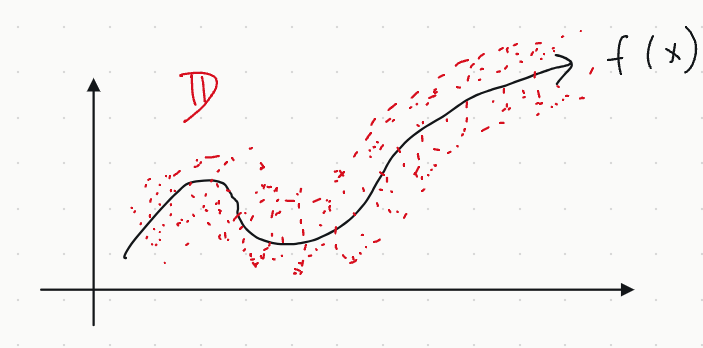
\includegraphics[width=0.5\textwidth]{homosk-mean-zero-centered}
		\caption{Depiction of zero mean-centered and mean independent $\Delta$,
		and homoskedasticity.}
		\label{fig:assumption-1-and-2}
	\end{figure}
	If $\delta$ is random from
	$\Delta$, then $y$ is also random from $Y$, so
	\begin{align}
		Y = f(\bm{x}) + \Delta
		\label{eqn:Y-rv-on-Delta}
	\end{align}
	and hence
	\begin{align}
		\mathbb{E}[Y \mid \bm{x}]
		&= \mathbb{E}[f(\bm{x}) + \Delta \mid \bm{x}]\nonumber\\
		&=\mathbb{E}[f(\bm{x})\mid \bm{x}] + \mathbb{E}[\Delta \mid \bm{x}]\nonumber\\
		&= f(\bm{x})
		\tag{by (I)}
	\end{align}
	Thus we call $f$ the \textbf{conditional expectation function (CEF)}.
	Let $g$ be a fitted model with $\mathbb{D}$, meaning
	\begin{align*}
		y &= g + e = g + \overbrace{(f - g) + \delta}^{e}\\
		e &= f - g + \delta
	\end{align*}
	Here $e$ is the residual, which has both misspecification and estimation.
	By Equation~\ref{eqn:assumption-1-mean-zero-independent}, we can say $e$ is a
	realization of a random variable $E$
	\begin{align*}
		Y &= g + \overbrace{(f - g) + \Delta}^{E}\\
		E &= (f-g) + \Delta = Y - g
	\end{align*}
	Let's predict on a new observation $\bm{x}_*$:
	\begin{align*}
		Y_* &= g(\bm{x}_*) + f(\bm{x}_*) - g(\bm{x}_*) + \Delta_*
	\end{align*}
	Then the associated error is
	\begin{align}
		E_* = f(\bm{x}_*) - g(\bm{x}_*) + \Delta_* = Y_* - g(\bm{x}_*)
		\label{eqn:error-rv}
	\end{align}
	See Figure~\ref{fig:prediction-error-rv}.
	\begin{figure}
		\centering
		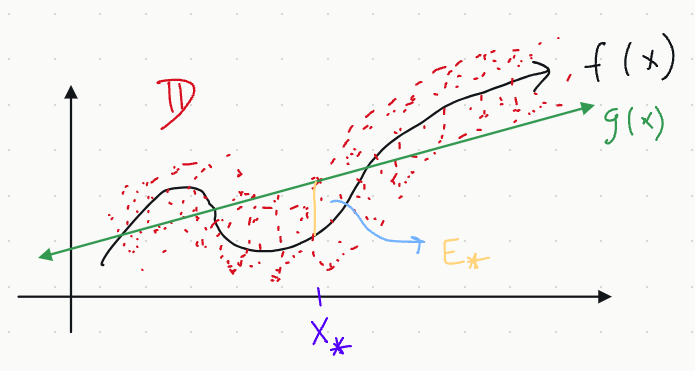
\includegraphics[width=0.6\textwidth]{prediction-error-random-variable}
		\caption{Depiction of random variable $E_*$}
		\label{fig:prediction-error-rv}
	\end{figure}
	Define the \textbf{bias} to be
	\begin{align}
		\text{Bias}(\bm{x}_*):
		&= \mathbb{E}[E_* \mid \bm{x}_*]
		\label{eqn:def-bias}
	\end{align}
	Then using Equation~\ref{eqn:error-rv}
	\begin{align*}
		\mathbb{E}[E_* \mid \bm{x}_*]
		& = \mathbb{E}[f(\bm{x}_*) - g(\bm{x}_*) + \Delta_* \mid \bm{x}_*]
		\tag{by ~\ref{eqn:error-rv}}\\
		& = f(\bm{x}_*) - g(\bm{x}_*) + \underbrace{\mathbb{E}[\Delta_* \mid \bm{x}_*]}_{0}
		\tag{$f$ and $g$ not random on $\bm{x}$}\\
		& = f(\bm{x}_*) - g(\bm{x}_*)
		\tag{by \ref{eqn:assumption-1-mean-zero-independent}}
	\end{align*}
	where $\mathbb{E}$ is expectation on $\Delta_*$ since that is what is random.
	Hence we have
	\begin{align}
		\text{Bias}(\bm{x}_*) = f(\bm{x}_*) - g(\bm{x}_*)
		\label{eqn:bias-f-minus-g}
	\end{align}
	Define \textbf{Mean-Squared Error (MSE)} by
	\begin{align}
		MSE(\bm{x}_*):
		&= \mathbb{E}[E_*^2 \mid \bm{x}_*]\label{eqn:-def-MSE}
	\end{align}
	which we can simplify to
	\begin{align*}
		\mathbb{E}[E_*^2 \mid \bm{x}_*]
		&=\mathbb{E}[(Y_* - g(\bm{x}_*))^2 \mid \bm{x}_*]\\
		&= \mathbb{E}[Y_*^2 - 2g(\bm{x}_*)Y_* + g(\bm{x}_*)^2 \mid \bm{x}_*]\\
		&= \mathbb{E}[Y_*^2 \mid \bm{x}_*] -2g(\bm{x}_*) \mathbb{E}[Y_* \mid \bm{x}_*] + g(\bm{x}_*)^2
		\tag{$g$ is not random in $\bm{x}_*$}\\
		&= \mathbb{E}[(f(\bm{x}_*) + \Delta_*)^2 \mid \bm{x}_*]
		- 2g(\bm{x}_*)\mathbb{E}[f(\bm{x}_*) + \Delta_* \mid \bm{x}_*] + g(\bm{x}_*)^2
		\tag{since $Y_* = f(\bm{x}_*) + \Delta_*$}\\
		&=  f(\bm{x}_*)^2 + 2 f(\bm{x}_*) \underbrace{\mathbb{E}[\Delta_* \mid \bm{x}]}_{0} +\underbrace{\mathbb{E}[\Delta_*^2 \mid \bm{x}_*]}_{\sigma^2}
		-2g(\bm{x}_*)f(\bm{x}_*) + \underbrace{\mathbb{E}(\Delta_* \mid \bm{x}_*)}_{0} + g(\bm{x}_*)^2
		\tag{$f$ is not random in $\bm{x}_*$}\\
		&=\sigma^2 + (f(\bm{x}_*) - g(\bm{x}_*))^2
		\tag{by \ref{eqn:assumption-1-mean-zero-independent} and \ref{eqn:assumption-2-homosk}}\\
		&=\sigma^2 +\left( \text{Bias}[\bm{x}_*]\right)^2
		\tag{by \ref{eqn:bias-f-minus-g}}
	\end{align*}
	If $g(\bm{x}) = f(\bm{x})$, then the only error is $\sigma^2$, called the
	\textbf{irreducible error}. This comes from $\Delta$, which we don't know.
	Recall bias results from misspecification and estimation.
	\subsection*{Allowing Randomness in Responses}
	Suppose now that $\mathbb{D}$ has randomness in the responses (not in $X$).
	Then $y_1,\ldots,y_n$ are realized are from $Y_1,\ldots,Y_n$ via
	$\Delta_1,\ldots,\Delta_n$, but $\bm{x}_1,\ldots,\bm{x}_n$ are constant. We make
	a third assumption, in addition to \ref{eqn:assumption-1-mean-zero-independent} and
	\ref{eqn:assumption-2-homosk}:
	\begin{center}
		(III) $\Delta_1,\ldots,\Delta_n$ are independent
	\end{center}
	What's different? The realizations of $\Delta$ are different, which means the
	models are different. There are uncountably-infinitely many data sets; what changes
	is the offset from $f(x)$. In the real world, you see one data set $\mathbb{D}$,
	and you would construct one $g(x)$. Each will be different because $g$ is
	a function of the algorithm, and since the $y$'s in $\mathbb{D}$ are random, $g$
	is in fact a realization of a corresponding random $G$:
	\begin{align*}
		G
		= \mathcal{A}(\mathbb{D}, \mathcal{H})
		= \mathcal{A}(\langle X, \vec{Y}\rangle, \mathcal{H})
	\end{align*}
	where $\vec{Y}$ is a (vector) random variable.
	Now consider the Mean-Squared Error again, defined as in \ref{eqn:-def-MSE}.
	In the following, $\mathbb{E}_{\mathbb{D}}$ means expectation involving
	randomness in the responses in $\mathbb{D}$ (as a consequence of randomness in
	$\Delta_1,\ldots,\Delta_n$), while $\mathbb{E}_{\Delta_*}$ means expectation
	involving randomness in $\Delta_*$:
	\begin{align*}
		MSE[\bm{x}_*] :
		&= \underset{\Delta_*, \mathbb{D}}{\mathbb{E}}[(Y_* - G(\bm{x}_*))^2 \mid \bm{x}_*, X]\\
		&= \underset{\Delta_*, \mathbb{D}}{\mathbb{E}}[Y_*^2 \mid \bm{x}_*, X]
		- 2\underset{\Delta_*, \mathbb{D}}{\mathbb{E}}[Y_* \cdot G(\bm{x}_*)\mid \bm{x}_*, X]
		+\underset{\Delta_*, \mathbb{D}}{\mathbb{E}}[G(\bm{x}_*)^2\mid \bm{x}_*, X]\\
		&= \mathbb{E}_{\Delta_*}[Y_*^2 \mid \bm{x}_*, X]
		-2\mathbb{E}_{\Delta_*}[Y_*\mid \bm{x}_*, X]\cdot \mathbb{E}_{\mathbb{D}}[G(\bm{x}_*)\mid \bm{x}_*, X]
		+\mathbb{E}_{\mathbb{D}}[G(\bm{x}_*)^2\mid \bm{x}_*, X]
		\tag{by independence, and $Y_*$ only random in $\Delta_*$, $G$ only random in $\mathbb{D}$}\\
		&=\sigma^2 + f(\bm{x}_*)^2
		- 2f(\bm{x}_*)\mathbb{E}_{\mathbb{D}}[G(\bm{x}_*)\mid \bm{x}_*, X]
		+\mathbb{E}_{\mathbb{D}}[G(\bm{x}_*)^2\mid \bm{x}_*, X]
		\tag{by \ref{eqn:Y-rv-on-Delta}, \ref{eqn:assumption-1-mean-zero-independent},
		\ref{eqn:assumption-2-homosk}}\\
		&=\sigma^2 + f(\bm{x}_*)^2
		- 2f(\bm{x}_*)\mathbb{E}_{\mathbb{D}}[G(\bm{x}_*)\mid \bm{x}_*, X]
		+\left(\mathbb{E}_{\mathbb{D}}[G(\bm{x}_*)\mid \bm{x}_*, X]\right)^2
		+\text{Var}[G(\bm{x}_*)\mid \bm{x}_*, X]
		\tag{by $\text{Var}[U] = \mathbb{E}[U^2]- \mathbb{E}[U]^2$}\\
		&=\sigma^2 + (f(\bm{x}_*) - \mathbb{E}_{\mathbb{D}}[G(\bm{x}_*)\mid \bm{x}_*, X])^2
		+\text{Var}[G(\bm{x}_*)\mid \bm{x}_*, X]
		\tag{by $(a-b)^2=a^2-2ab+b^2$}\\
		&=\sigma^2 + (\mathbb{E}_{\mathbb{D}}[f(\bm{x}_* - G(\bm{x}_*)\mid \bm{x}_*, X])^2
		+\text{Var}[G(\bm{x}_*)\mid \bm{x}_*, X]
		\tag{$f$ is not random on $\mathbb{D}$}\\
		&=\sigma^2 + \left(\text{Bias}[G(\bm{x}_*)]\right)^2 + \text{Var}[G(\bm{x}_*)]
		\tag{by \ref{eqn:def-bias}}
	\end{align*}
	In summary, we have
	\begin{align}
		MSE[\bm{x}_*] =
		\sigma^2 + \left(\text{Bias}[G(\bm{x}_*)]\right)^2 + \text{Var}[G(\bm{x}_*)]
		\label{eqn:bias-var-decomp}
	\end{align}
	Equation~\ref{eqn:bias-var-decomp} is called the \textbf{Bias-Variance decomposition},
	or \textbf{Bias-Variance trade-off}. Intrigued by the name, it is natural to ask
	whether there is in fact a trade-off between bias and variance, and in what sense.
	\begin{itemize}
		\item If you define ``trade-off" as a \textit{zero-sum game}, then the answer
		is \textit{no}, since there are algorithms $\mathcal{A}$ that reduce \textit{both}
		bias and variance simultaneously.
		\item If by ``trade-off" you instead mean \textit{decomposition}, then yes,
		there is a ``trade-off", as both terms appear in Equation~\ref{eqn:bias-var-decomp}.
	\end{itemize}
	See Figure~\ref{fig:bias-variance-tradeoff}.
	\begin{figure}
		\centering
		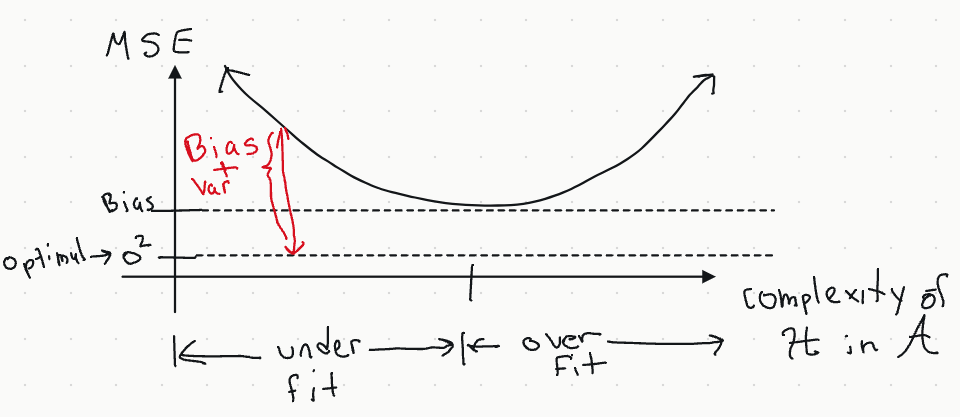
\includegraphics[width=0.7\textwidth]{bias-variance-tradeoff}
		\caption{Depiction of bias-variance decomposition.}
		\label{fig:bias-variance-tradeoff}
	\end{figure}
	\subsection*{Allowing Randomness in Covariates}
	We make another generalization: randomness in the $\bm{x}$'s. Thus,
	further assume $\bm{x}_1,\bm{x}_2,\ldots,\bm{x}_n,\bm{x}_*$ are random,
	drawn from random variable $\vec{X}$. Before, we calculated the MSE
	over a fixed $\bm{x}$, but now, we do so over \textit{all} observations:
	\begin{align}
		MSE :
		&= \mathbb{E}_{\vec{X}}[MSE[\bm{x}]]\nonumber\\
		&= \mathbb{E}_{\vec{X}}[\sigma^2 + (\text{Bias}[G(\bm{x}_*)])^2 + \text{Var}[G(\bm{x}_*)]]\nonumber
		\tag{by \ref{eqn:bias-var-decomp}}\\
		&=\sigma^2 + \mathbb{E}_{\vec{X}}[(\text{Bias}[G(\bm{x}_*)])^2]
		+ \mathbb{E}_{\vec{X}}[\text{Var}[G(\bm{x}_*)]]
		\label{eqn:general-bias-var-decomp}
	\end{align}
	Equation~\ref{eqn:general-bias-var-decomp} is the \textbf{general version of
	the Bias-Variance Decomposition}.
	
	How can we reduce the values of the last two terms in
	Equation~\ref{eqn:general-bias-var-decomp}? We can make the bias $0$ by
	making $\mathcal{H}$ complex, effectively overfitting. Hence, bias would
	decrease, but the variance term will in increase.\footnote{Recall setting (I) of our
		model selection procedure, where we have $M$ pre-specified modeling procedures
		and we choose the optimal $m_*$? This may be a good place to apply it.}
	Consider the \textbf{model average}:
	\begin{align*}
		g_{avg} := \frac{\sum_{m=1}^{M}g_m}{M}
	\end{align*}
	This can be smart if all $M$ models are known to be good, since this can
	reduce variation. On the down side, we give up interpretability (suppose,
	for example, they were linear models). Let's examine the bias-variance decomposition
	for $g_{avg}$ (henceforth we use $G_{avg}$, since $g_{avg}$ is realized from it):
	\begin{align}
		MSE :
		&= \sigma^2 + \mathbb{E}[\text{Bias}[G_{avg}(\bm{x}_*)]^2]
		+\mathbb{E}[\text{Var}[G_{avg}(\bm{x}_{*})]]\nonumber\\
		&= \sigma^2 + \mathbb{E}\left[
			\left(
				f - \frac{G_1 + \cdots + G_M}{M} 
			\right)^2
		\right]
		+ \mathbb{E}\left[\text{Var}\left[\frac{G_1 + \cdots + G_M}{M}\right]\right]
		\tag{by \ref{eqn:def-bias}}
		\nonumber\\
		&= \sigma^2 + \mathbb{E}\left[
			\left(\frac{(f - G_1) + \cdots + (f - G_M)}{M}\right)^2
		\right]
		+ \frac{1}{M^2}\cdot \mathbb{E}\left[\text{Var}\left[G_1 + \cdots + G_M \right]\right]
		\label{eqn:mse-Gavg-in-progress}
	\end{align}
	In our first attempt to simplify this expression, we make the following assumptions:
	\begin{enumerate}[label=(\roman*)]
		\item The bias of each model is the same: $\text{Bias}[G_1]=\cdots=\text{Bias}[G_M]$.
		\item The models $G_1,\ldots,G_M$ are independent.
		\item The variance of each model is the same:
		$\text{Var}[G_1] = \cdots = \text{Var}[G_M]$.
	\end{enumerate}
	Then continuing from Equation~\ref{eqn:mse-Gavg-in-progress}:
	\begin{align*}
		MSE &=\sigma^2 + \mathbb{E}[\left(\text{Bias}[G_1]\right)^2]
		+\mathbb{E}\left[
		\frac{1}{M}\cdot \text{Var}[G_1]
		\right]
		\tag{by (i) and (iii)}\\
		&\to \sigma^2
		\tag{let $M\to\infty$ and use $\mathcal{H}$ to overfit}
	\end{align*}
	What do we make of this? Assumption (ii) said that we have independent models,
	which is fake! Moreover, in the real world, we have one data set $\mathbb{D}$,
	and one $g$, so the $g$'s cannot be independent. However the fact that we
	eliminated bias by overfitting is reasonable (we can use trees with small $N_0$).
	We need to come up with a reasonable way to reduce the variance term that does
	not use assumption (ii).
	\subsection*{Review of Correlation and Covariance}
	Recall from introductory probability that the \textbf{covariance}
	of a pair of random variables $X_i$ and $X_j$ is given by
	\begin{align*}
		\sigma_{ij} := \text{Cov}[X_i,X_j] := \mathbb{E}[X_i\cdot X_j] - \mu_i\mu_j
	\end{align*}
	where $\mu_i = \mathbb{E}[X_j]$.
	Meanwhile, the \textbf{correlation} of random variables $X_i$ and $X_j$
	is given by
	\begin{align*}
		\rho_{ij} := \text{Corr}[X_i,X_j] := \frac{\text{Cov}[X_i,X_j]}{\text{SD}[X_i]\cdot \text{SD}[X_j]}
	\end{align*}
	where SD stands for standard deviation.
	The covariance is a measure of how much $X_i$ and $X_j$ change together,
	yielding a positive value if both tend to increase together, and negative
	if both tend to decrease together. The correlation $\rho_{ij}$ is a normalized
	version of covariance, with $\rho\in [-1, 1]$.
	
	Let $X_1,\ldots,X_n$ be random variables. Assume $\sigma_{ij}$ is the same for all
	ordered pairs $i\neq j$ (of which there are $n^2 - n$), and that
	$\sigma^2 = \sigma_1^2 = \cdots = \sigma_n^2$. Then
	\begin{align}
		\rho = \frac{\sigma_{ij}}{\sigma^2}
		\label{eqn:corr-equal-cov-and-var}
	\end{align}
	Define the mean of the given random variables
	\begin{align*}
		\overline{X} := \frac{\sum_{i=1}^{n}X_i}{n}
	\end{align*}
	Then
	\begin{align*}
		\text{Var}[\overline{X}]
		&= \frac{1}{n^2}\text{Var}\left[\sum_{i=1}^{n}X_i\right]\\
		&= \frac{1}{n^2}\left(
		\sum_{i=1}^{n}\text{Var}[X_i] + \sum_{i\neq j}\text{Cov}[X_i,X_j]
		\right)\tag{derived in intro probability}\\
		&= \frac{1}{n^2}\left(
		n\sigma^2 + (n^2-n)\sigma_{ij}
		\right)\tag{assuming equal $\sigma_{ij}$}\\
		&= \frac{1}{n}\left(
		\sigma^2 + (n - 1)\sigma^2 \rho
		\right)
		\tag{by \ref{eqn:corr-equal-cov-and-var}}\\
		&=\sigma^2\rho + \frac{\sigma^2(1-\rho)}{n}
	\end{align*}
	In summary, if $\sigma_{ij}$ is the same for all $X_i, X_j$,
	and their variances are all equal, we have
	\begin{align}
		\text{Var}[\overline{X}] = \sigma^2\rho + \frac{\sigma^2 (1-\rho)}{n}
		\label{eqn:variance-Xbar}
	\end{align}
	\subsection*{Dependent Models}
	Continuing to assume equal bias for models $G_1,\ldots,G_M$, that
	the variance of each model is the same, and replacing assumption (ii)
	with the assumption that
	the covariance of each pair of models is the same:
	\begin{align*}
		MSE :
		&=\sigma^2 + \mathbb{E}[\text{Bias}[G_{avg}(\bm{x}_*)]^2]
		+\mathbb{E}[\text{Var}[G_{avg}(\bm{x}_{*})]]\\
		&=\sigma^2 + \mathbb{E}[\text{Bias}[G_{1}(\bm{x}_*)]^2]
		+\mathbb{E}\left[\text{Var}[G_{1}(\bm{x}_{*})]\cdot \rho +
		\frac{\text{Var}[G_1]\cdot (1-\rho)}{M}
		 \right]
		 \tag{by \ref{eqn:variance-Xbar}}\\
 		&\to\sigma^2 + \mathbb{E}[\text{Bias}[G_1(\bm{x}_*)]^2] +
 		\mathbb{E}[\rho \cdot \text{Var}[G_1]]
 		\tag{let $M\to\infty$}\\
 		&\to\sigma^2+\rho \cdot \mathbb{E}[\text{Var}[G_1]]
 		\tag{let $\mathcal{A}$ overfit, bias becomes 0}\\
 		&<\sigma^2 + \mathbb{E}[\text{Var}[G_1]]
 		\tag{since $\rho \leq 1$, plus assume $\rho>0$}
	\end{align*}
	The last equation is the MSE for \textit{one} overfit model, whereas
	the equation that precedes it is the MSE for $M$ overfit models.
	We cannot make the models independent, but can we make them dependent
	such that their dependence is nontrivially less than 1? This would
	help reduce the error in the variance term.
	\section*{Bootstrap Aggregation}
	In 1994, \textbf{Bootstrap Aggregation (Bagging)} was invented by
	Breiman. How do we make $\rho$ smaller than, say, 0.9? Even better,
	smaller than 0.2, which would be close to the theoretical minimum
	for the MSE (which is $\sigma^2$)?
	
	Let's sample the results of $\mathbb{D}$ a total of $n$ times with replacement
	where $n$ is the number of data points in $\mathbb{D}$.
	The probability that a given row is chosen on any given trial is
	$\frac{1}{n}$, and hence the probability that it is omitted is
	$\frac{n-1}{n}=1-\frac{1}{n}$. Thus, the probability that a given
	row is omitted in all $n$ tries is
	\begin{align*}
		\left(1 - \frac{1}{n}\right)^n\approx \frac{1}{e}\approx \frac{1}{3}
	\end{align*}
	This is called a \textbf{bootstrap sample}. Let's take $M$ bootstrap samples.
	With this we can compute $M$ overfit models
	\begin{align*}
		g_1 = \mathcal{A}(\mathbb{D}_1,\mathcal{H}),\ldots,
		g_M = \mathcal{A}(\mathbb{D}_M, \mathcal{H})
	\end{align*}
	Then we use the average of them, $g_{avg}$. Since all $g$'s are built
	from the same $\mathbb{D}$, they will be a little correlated, and yet
	they will all be a little different because they are built from a different
	$\mathbb{D}_m$. Thus $\rho$ will not be zero and will be a little less
	than $1$. Typically, we bag trees with small $N_0$ (for example $N_0 = 1$),
	and we let $M$ be as large as practically allowable.
\end{document}